\begin{frame}
	\frametitle{Volume and Balance adjustment}
	
    \begin{itemize}
		\item
		\item Audio signal adjustment
		\item Storage of system levels
		\item
		\item
    \end{itemize}
	
	\begin{figure}
		\centering
		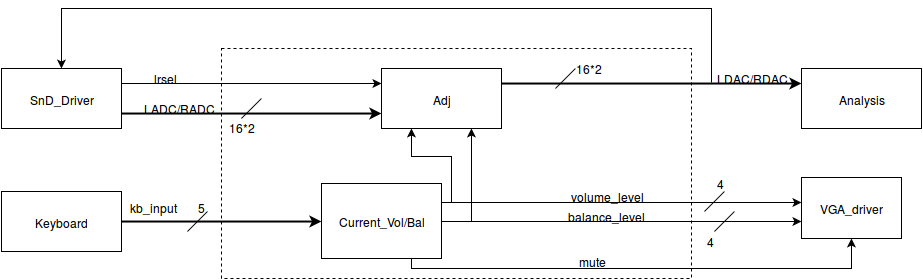
\includegraphics[scale=.3]{volbal}
	\end{figure}

\end{frame}

\begin{frame}
	\frametitle{Volume and Balance adjustment}
	\framesubtitle{Current\_Vol\_Bal}
	
	\begin{itemize}
		\item Volume: 0 to 10
		\item Balance: -8 to 8
		\item Legality example: \\
		\item 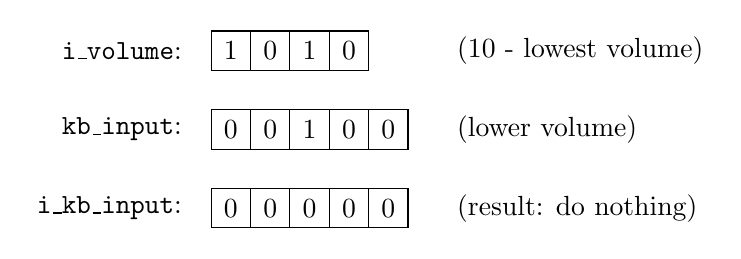
\begin{tikzpicture}[y=.5 cm, x=.5 cm]
				\draw(4.5,4.5) node[anchor=east]{\texttt{i\_volume}:};
				\draw(4.5,2.5) node[anchor=east]{\texttt{kb\_input}:};
				\draw(4.5,0.5) node[anchor=east]{\texttt{i\_kb\_input}:};
				
				\draw(5,4) rectangle (9,5);
				\draw(5,2) rectangle (10,3);
				\draw(5,0) rectangle (10,1);
				
				\foreach \x in {6,...,9}
				\draw (\x, 0 ) -- ( \x, 1 );
				
				\foreach \x in {6,...,9}
				\draw (\x, 2 ) -- ( \x, 3 );
				
				\foreach \x in {6,...,8}
				\draw (\x, 4 ) -- ( \x, 5 );
				
				\draw(5.5,4.5) node{1};
				\draw(6.5,4.5) node{0};
				\draw(7.5,4.5) node{1};
				\draw(8.5,4.5) node{0};
				
				\draw(5.5,2.5) node{0};
				\draw(6.5,2.5) node{0};
				\draw(7.5,2.5) node{1};
				\draw(8.5,2.5) node{0};
				\draw(9.5,2.5) node{0};
				
				\draw(5.5,0.5) node{0};
				\draw(6.5,0.5) node{0};
				\draw(7.5,0.5) node{0};
				\draw(8.5,0.5) node{0};
				\draw(9.5,0.5) node{0};
				
				\draw(11,4.5) node[anchor=west]{(10 - lowest volume)};
				\draw(11,2.5) node[anchor=west]{(lower volume)};
				\draw(11,0.5) node[anchor=west]{(result: do nothing)};
				
		\end{tikzpicture}	
	\end{itemize}
	
\end{frame}

\begin{frame}
	\frametitle{Volume and Balance adjustment}
	\framesubtitle{Volume\_Adjustment}

	\begin{itemize}
		\item Logarithmic scaling $$A_{adj} = A_{in} \cdot (1/\sqrt{2})^n$$
		\item Output range: -30 to 0 dB
		\item Implemented using a state machine
	\end{itemize}	
	
\end{frame}

\begin{frame}
	\frametitle{Volume and Balance adjustment}
	\framesubtitle{Balance\_Adjustment}
	
	\begin{itemize}
		\item Linear scaling $$A_{l\_out} = \frac{8 - m}{8} \cdot A_{l\_adj}\ \ ,\ A_{l\_out} = A_{l\_adj}\ for\ m < 0$$ $$A_{r\_out} = \frac{8 - |m|}{8} \cdot A_{r\_adj}\ \ ,\ A_{r\_out} = A_{r\_adj}\ for\ m > 0$$
		\item Controlled by \texttt{volume\_done} and \texttt{lrsel}.
	\end{itemize}
	
\end{frame}

%	Our system can scale audio input both logarithmically for volume and linearly
%	for channel balance adjustment. The module responsible for these tasks is 
% 	the Vol_Bal module.
%	--- Most of you are familiar with the Sound Lab enviroment, and in comparison, 
%	our Vol_Bal assumes the logistic position of the Application module.
% 	--- Vol_Bal also stores the system level settings within its submodule
%	Current_Vol_Bal, which updates via the kb_input signal from the Keyboard module.

%	Now, on to the implementation.
%	
%	To start with, the Current_Vol_Bal module faces merely one challenge: 
%	When we update its registers, we need to stay on the legal range of values.
%	For volume, this is 0 to 10. For balance, -8 to 8. This is accomplished with
%	simple AND/OR logic. A '1' bit in the kb_input-vector only stays '1' if the relevant
%	system level is not already its legal max or min value. After that check, we update
%	accordingly.
%	--- These register outputs are then used for both the adjustments locally, and as
%	information for VGA_Driver so that the settings can be rendered on screen.

%	Moving on, Volume_Adjustment adjusts the LADC/RADC input, scaling it down
%	logarithmically in accordance with the formula below.
%	--- Every multiplication with the inverse square root of 2 results in a signal
%	reduction of approximately 3 dB. We do this n times where n is the volume level,
%	meaning we can change the audio signal on the range -30 to 0 dB.
%	--- To accomplish a varied amount of "multiplications", we use a state machine
%	that remains in an amplitude reduction state based on the value of system volume.
%	--- lrsel triggers the state machine and a "volume done" signal is forwarded when 
%	adjustment is complete.

%	Finally, the Balance_Adjustment submodule. Balance needs to perform linear
%	balance scaling according to THESE ***point at slide*** formulas.
%	The implementation of these does not require a state machine, but we need to
%	keep the current m value updated, based on our system balance level. A process
%	statement does this with ease, using lrsel as an aide and following the rules
%	in the listed functions.
%	--- The volume_done signal is used as a ready-signal for the adjusted audio input,
%	and the resulting output is sent back to SndDriver and to the post-processing Analysis 	%	module.

%	Now, X will talk about Y.